\documentclass[11pt]{amsart}
\usepackage[margin=1.1in]{geometry}
\usepackage{amsmath,amssymb,amsthm,mathtools}
\usepackage{enumitem}
\usepackage{tikz}
\usepackage[hidelinks]{hyperref}

\emergencystretch=1.5em
\newtheorem{theorem}{Theorem}[section]
\newtheorem{lemma}[theorem]{Lemma}
\newtheorem{corollary}[theorem]{Corollary}
\newtheorem{proposition}[theorem]{Proposition}
\theoremstyle{definition}
\newtheorem{definition}[theorem]{Definition}
\newtheorem{remark}[theorem]{Remark}

\newcommand{\cells}{\operatorname{cells}}
\newcommand{\Core}{\operatorname{Core}}
\newcommand{\Res}{\operatorname{Res}}
\newcommand{\Spare}{\operatorname{Spare}}
\newcommand{\Own}{\operatorname{Own}}
\newcommand{\blank}{\operatorname{blank}}
\newcommand{\sel}{\operatorname{sel}}
\newcommand{\pop}{\operatorname{pop}}
\newcommand{\base}{\operatorname{base}}
\newcommand{\rate}{\operatorname{rate}}
\newcommand{\cost}{\operatorname{cost}}

\title[God's number of the sliding puzzle]{God's number of the $n\times n$ sliding puzzle is $n^3+O(n^2\log n)$}
\date{}

\begin{document}

\begin{abstract}
Let $\mathcal G(n)$ be the largest distance, measured in single slides, between two
mutually reachable configurations of the $n\times n$ sliding puzzle (the
$(n^2-1)$-puzzle). A simple potential argument shows $\mathcal G(n)\ge n^3-O(n)$. We
prove the matching upper bound $\mathcal G(n)\le n^3+O(n^2\log n)$. The algorithm routes every tile
from its starting cell up through a hierarchy of nested ``star routers'' to the
centre of the board, and back down to its home. Tiles move in pipelined queues in which one
slide advances one tile by one cell, so the total cost is
twice the sum of the distances of all cells to the centre, which is at most
$n^3$, plus $O(n^2)$ for each of the $O(\log n)$ levels of the hierarchy.
\end{abstract}

\maketitle

\section{Introduction}

The $n\times n$ sliding puzzle has $n^2-1$ numbered tiles and one empty cell, the
\emph{blank}, on an $n\times n$ grid. A \emph{move} (or \emph{slide}) moves a tile
adjacent to the blank into the blank. Two configurations are \emph{connected} if
one can be turned into the other by moves. \emph{God's number} $\mathcal G(n)$ is the
maximum, over connected pairs, of the least number of moves joining them.

\begin{theorem}\label{thm:main}
There are constants $C_\star$ and $N_\star$ such that for every $n\ge N_\star$, any two connected
configurations of the $n\times n$ puzzle are joined by at most
\[
n^3+C_\star\,n^2(\log_{16} n+1)
\]
moves. Hence $\mathcal G(n)=n^3+O(n^2\log n)$.
\end{theorem}

The leading term cannot be improved.

\begin{remark}[Lower bound]\label{rem:lower}
Fix a target board. A move changes the sum, over all non-blank tiles, of the Manhattan distance between a tile's
cell and its cell in the target by exactly one. Consider the board in which the tile whose target cell is $x$ sits at the point reflection of $x$
through the centre of the board. If it is not connected to the target, exchange two
adjacent non-blank tiles: by the parity criterion of Johnson and Story~\cite{johnsonstory} (two boards are connected exactly when
the parity of the cell permutation between them equals the parity of the blank's displacement) this makes it connected,
and it changes the total by $O(1)$. Leaving out the blank's own term, which is $O(n)$, the total is at least
$\sum_{0\le i,i'<n}\bigl(|2i-n+1|+|2i'-n+1|\bigr)-O(n)$. The sum is $n^3$ for even $n$ and
$n^3-n$ for odd $n$. Hence $\mathcal G(n)\ge n^3-O(n)$.
\end{remark}

\subsection*{The idea}
Moving the blank once around a closed loop of cells shifts every tile on the loop by one
cell, at a cost of one move per tile (Lemma~\ref{lem:walk}). A
long loop is therefore a conveyor belt that transports tiles at an amortised cost of
one move per tile per cell. If every tile could travel from its start to the
centre of the board and from the centre to its home along such belts, the total cost would be
$2\sum_x d(x,\text{centre})\approx n^3$, where $d$ is the Manhattan distance and $x$ ranges over the cells.

To realise this we split the board recursively into a hierarchy. Each node of
the hierarchy is a square. A non-leaf node is a \emph{star router}: a small hub, and $b^2$ child
squares (we take $b=16$), each connected to the hub by a pair of conveyor
belts (an export lane and a delivery lane). Tiles leave a child through its
export lane and enter it through its delivery lane. A node talks to its parent
through a narrow interface. It is fed one tile at a time and hands back one
tile in exchange (Section~\ref{sec:regions}). Each level of the hierarchy wastes
only $O(T^2)$ moves at a node of side $T$, beyond the conveyor cost, and there are
$O(\log n)$ levels. This gives $n^3+O(n^2\log n)$.

The difficulty is to make this precise. A node must hand out a tile before
it has received the tiles that belong in it. It must keep its children supplied
with exchange tiles. It must never get stuck. And it must account for every
move. The interface of Section~\ref{sec:regions} isolates exactly what a node
promises to its parent. The core of the paper (Section~\ref{sec:star}) shows that a star
router whose children keep these promises keeps them too, with an explicit cost.

\subsection*{Plan of the paper}
Section~\ref{sec:prelim} collects elementary facts about moves.
Section~\ref{sec:regions} defines \emph{regions}, the interface every node
implements. Section~\ref{sec:leaf} treats the leaves of the hierarchy.
Section~\ref{sec:star} proves that a star router over regions is a region, and
bounds its cost. Section~\ref{sec:tree} builds the hierarchy (the \emph{corner
tree}) and solves its cost recursion. Section~\ref{sec:root} builds the root,
a star over four quadrant trees around the centre of the board, and proves
Theorem~\ref{thm:main}.

\subsection*{Formal verification}
The complete argument, with explicit constants, has been formalised in the Lean~4 proof assistant
with the Mathlib library. The formalisation uses only the standard axioms (propositional
extensionality, choice and quotient soundness). This paper is self-contained and
does not depend on it. We suppress all specific constants.

\section{Preliminaries}\label{sec:prelim}

\subsection{Boards and moves}
Cells are pairs $(i,i')$ with $0\le i,i'<n$ (row, column). Two cells are
\emph{adjacent} if they differ by one in exactly one coordinate. The distance
$d(x,y)$ between $x=(i,i')$ and $y=(k,k')$ is the Manhattan distance $|i-k|+|i'-k'|$. A \emph{board} is a bijection
$B$ from cells to tiles $\{0,1,\dots,n^2-1\}$, where $0$ is the blank;
$\blank(B)=B^{-1}(0)$. We say $B(x)$ is the \emph{content} of cell $x$. A move
exchanges the contents of $\blank(B)$ and an adjacent cell. A \emph{path} is a
sequence of moves; its length is its number of moves. All costs in this paper
are lengths of paths. We call a path \emph{blank-returning} if the blank ends
where it started.

A blank-returning path changes $B$ into $B'$ with $B'(\pi(x))=B(x)$ for a
permutation $\pi$ of cells fixing $\blank(B)$: the \emph{effect} of the path. We say the path
\emph{moves the content of $x$ to $\pi(x)$}. A $3$-cycle $(a\ b\ c)$ moves the content of
$a$ to $b$, of $b$ to $c$, and of $c$ to $a$.

\begin{lemma}[walks]\label{lem:walk}
Let $c_0,c_1,\dots,c_k$ be distinct cells, each adjacent to the next, with the
blank at $c_0$. Moving the blank along them (cost $k$) moves the content of
$c_i$ to $c_{i-1}$ for $1\le i\le k$, and leaves the blank at $c_k$. If $c_k$ is adjacent to
$c_0$ and the blank continues to $c_0$ (total cost $k+1$, a \emph{loop}), the contents of
$c_2,\dots,c_k$ move one step back along the loop and the content of $c_1$ moves to
$c_k$. In both cases no other cell changes.
\end{lemma}

\begin{proof}
Each move exchanges the blank with the next cell of the walk.
\end{proof}

\begin{lemma}[conjugation]\label{lem:conj}
Let $\sigma$ be a path taking the blank from $z$ to $z'$, and $\bar\sigma$ the same moves in reverse order.
Let $\eta$ be a blank-returning path from $z'$ whose effect fixes every cell outside a set $U\ni z'$. Then
$\sigma\eta\bar\sigma$ is blank-returning, has length $2|\sigma|+|\eta|$, and its effect fixes every cell $x$ whose
content $\sigma$ does not carry into $U$. If moreover $\sigma$ leaves every cell of $U\setminus\{z'\}$ with its content, then the
effect of $\sigma\eta\bar\sigma$ agrees with that of $\eta$ on $U\setminus\{z'\}$.
\end{lemma}

\begin{proof}
Let $\hat\sigma$ be the permutation of cells, blank included, by which $\sigma$ moves contents, and $\hat\eta$
that of $\eta$. Then $\bar\sigma$ acts by $\hat\sigma^{-1}$ and the composite acts by $\hat\sigma^{-1}\hat\eta\hat\sigma$,
which fixes every $x$ with $\hat\sigma(x)\notin U$. If $\hat\sigma$ fixes $U\setminus\{z'\}$ pointwise, then for $x\in U\setminus\{z'\}$
we have $\hat\eta(x)\in U\setminus\{z'\}$, because $\hat\eta$ fixes $z'$, so the composite maps $x$ to $\hat\eta(x)$.
\end{proof}

The effect of a path on cells does not depend on the contents of the cells, only on the route of the blank. So it is harmless
for a path to pass temporarily through cells used by some other structure, as long as its net effect restores them.
We use Lemma~\ref{lem:conj} constantly in the following form: walk the blank along a walk, do an operation
that changes only cells off the walk (other than the walk's end, where the blank is), and walk back. Every
cell of the walk is then restored.

\subsection{Local permutations}
A \emph{square} of side $s$ is a set of cells $\{(r_0+i,c_0+j):0\le i,j<s\}$.
A path stays \emph{inside} a square if the blank never leaves it; such a path
only changes cells of the square.

\begin{lemma}[$3$-cycles]\label{lem:three}
Let $\mathcal S$ be a square of side $s\ge 6$ containing the blank, and let $a,b,c$ be distinct
non-blank cells of $\mathcal S$. There is a blank-returning path inside $\mathcal S$, of length $O(s)$, whose
effect is the $3$-cycle $(a\ b\ c)$. The same holds for $(a\ c\ b)$.
\end{lemma}

\begin{proof}
Use coordinates $(i,i')\in[0,s)^2$ in $\mathcal S$. A \emph{rectangle} is a set $[i_0,i_1]\times[j_0,j_1]$ of cells of $\mathcal S$.

\emph{Transport.} Let $U$ be a rectangle with both sides at least $3$ that contains the blank and a tile $t$.
Then $t$ can be moved to any cell of $U$ by $O(s)$ moves inside $U$. Indeed, to push $t$ one step in some
direction, bring the blank to the cell ahead of $t$ without passing through $t$. This is possible
because $U$ minus one cell is connected, and it costs $O(s)$ the first time. Then exchange. To push again in the same
direction, the blank, now just behind $t$, goes round $t$ through a neighbouring row or column of $U$ (one exists
because the sides are at least $3$) in $4$ moves. At the bend of an L-shaped route the blank walks, inside $U$ and avoiding $t$, to the cell ahead of $t$ in
the new direction ($O(s)$ moves). Moving $t$ along an L-shaped route therefore costs $O(s)$. (This is the elementary step of
the classical row-by-row algorithm; see e.g.~\cite{parberry}.)

\emph{Staging.} Let $t_1,t_2,t_3$ be the tiles at $a,b,c$. We place them at $(0,0)$, $(0,1)$, $(1,1)$ in turn.
\begin{enumerate}[nosep]
\item Transport $t_1$ to $(0,0)$ inside $U=\mathcal S$.
\item Let $U'=[1,s-1]\times[0,s-1]$, which avoids $(0,0)$. If $t_2$ is in row $0$, bring the blank below it
  (avoiding $(0,0)$ and $t_2$) and push $t_2$ down. Bring the blank into $U'$ without moving $t_2$ or $t_1$: if it is in row $0$, walk it along row $0$ to a column other than $0$ and other
than $t_2$'s (one exists since $s\ge4$), and step down. Transport $t_2$ inside $U'$
  to $(1,1)$. Move the blank, inside $U'$ and then up through column $2$, to $(0,2)$, then to $(0,1)$; this passes
  neither $(0,0)$ nor $(1,1)$. Push $t_2$ up into $(0,1)$; the blank is now at $(1,1)$.
\item In the same way, using $U'$, which avoids $(0,0)$ and $(0,1)$, transport $t_3$ to $(2,1)$. If $t_3$ is in row $0$, first push it
  down; when bringing the blank out of row $0$, walk it only through columns $\ge2$ other than $t_3$'s. Bring the blank to $(1,1)$ avoiding $(2,1)$ and row $0$, and push $t_3$ up. The blank is now at $(2,1)$;
  move it to $(2,0)$ and then to $(1,0)$.
\end{enumerate}
Each step costs $O(s)$ moves inside $\mathcal S$ and never disturbs the tiles already placed. Call the whole path $\sigma$.
Afterwards $(0,0),(0,1),(1,1)$ hold $t_1,t_2,t_3$ and the blank is at $(1,0)$.

\emph{Gadget.} Moving the blank round the block, $(1,0)\to(0,0)\to(0,1)\to(1,1)\to(1,0)$, moves $t_1$ to $(1,1)$,
$t_3$ to $(0,1)$ and $t_2$ to $(0,0)$ (Lemma~\ref{lem:walk}). Going round the other way does the inverse.

\emph{Conjugation.} The path $\sigma$, then the gadget, then $\bar\sigma$, has the effect $\hat\sigma^{-1}\hat\eta\hat\sigma$
(Lemma~\ref{lem:conj}), where $\hat\eta$ is the gadget's $3$-cycle on the staged cells. This is a $3$-cycle on $a,b,c$.
The two directions of the gadget give the two $3$-cycles $(a\ b\ c)$ and $(a\ c\ b)$.
\end{proof}

\begin{corollary}[double transpositions]\label{cor:double}
In the setting of Lemma~\ref{lem:three}, for distinct non-blank cells $a,b,c,d$ of $\mathcal S$, the
exchange of the contents of $a$ and $b$ together with that of $c$ and $d$ costs
$O(s)$ moves, blank-returning, inside $\mathcal S$.
\end{corollary}

\begin{proof}
Do the $3$-cycle $(b\ c\ d)$, then $(a\ b\ c)$.
\end{proof}

A single exchange of two contents is impossible with the blank returning (by
the parity argument below). Every exchange we need is therefore paired with an exchange of
two cells whose contents we do not care about. We call these two cells a \emph{parity pair}.

\begin{lemma}[local placement]\label{lem:place}
Let $\mathcal S$ be a square of side $s\ge6$, and $\mathcal R\subseteq\mathcal S$ a set of cells containing the blank. Let
$Z\subseteq \mathcal R\setminus\{\blank\}$ with $|\mathcal R|\ge|Z|+3$, and let $\psi$ assign distinct non-blank tiles to the cells of $Z$,
each currently in a cell of $\mathcal R$. Then a blank-returning path of length $O(s\,|Z|)$ makes every $f\in Z$ contain
$\psi(f)$, and changes no cell outside $\mathcal R$.
\end{lemma}

\begin{proof}
Fix two cells $y_1\neq y_2$ of $\mathcal R\setminus(Z\cup\{\blank\})$. Treat the cells of $Z$ one at a time. If $f$ does not yet
hold $\psi(f)$, let $y$ be the cell holding $\psi(f)$. Then $y$ is not the blank cell, and it is not a cell treated
earlier, since $\psi$ is injective. Pick $y'\in\{y_1,y_2\}$ with $y'\ne y$ and perform the $3$-cycle $(y\ f\ y')$ by
Lemma~\ref{lem:three}. This places $\psi(f)$ in $f$ and changes only $y,f,y'$, none of them treated earlier.
\end{proof}

\subsection{Parity and global clean-up}

\begin{lemma}[parity]\label{lem:parity}
If $B$ and $B'$ are connected and have their blank in the same cell, then the permutation
of cells carrying contents of $B$ to contents of $B'$ is even.
\end{lemma}

This is the classical criterion of Johnson and Story~\cite{johnsonstory}; we only need the easy direction.
\begin{proof}
Colour the cells like a chessboard. Every move changes the colour of the blank cell,
so a path from $B$ to $B'$ has even length. Each move is a transposition of two
contents, so the permutation is a product of an even number of transpositions.
\end{proof}

\begin{lemma}[clean-up]\label{lem:cleanup}
Let $n\ge6$, and let $B,B'$ be connected boards with the same blank cell that differ on a set
$S$ of cells. Then they are joined by a path of length $O(n|S|)$.
\end{lemma}

\begin{proof}
The permutation $\varphi$ carrying $B$'s contents to $B'$'s is supported on $S$ and is
even (Lemma~\ref{lem:parity}). If $\varphi$ has a cycle of length at least $3$, one $3$-cycle
places two of its contents correctly. Otherwise $\varphi$ is a product of at least two disjoint
transpositions, and two $3$-cycles fix four cells (Corollary~\ref{cor:double}). By Lemma~\ref{lem:three},
applied with the whole board as the square, each $3$-cycle costs $O(n)$; it avoids the blank cell, which is
already correct. The support shrinks by at least one per $3$-cycle.
\end{proof}

\begin{lemma}[gathering]\label{lem:gather}
Let $n\ge6$. Let $\mathcal K$ be a set of $k$ tiles containing $0$, and $\mathcal R$ a set of $k$ cells
containing the blank of $B$, with $2k<n^2$. A path of length $O(nk)$, keeping the blank cell, makes
the tiles of $\mathcal K$ occupy exactly the cells of $\mathcal R$.
\end{lemma}

\begin{proof}
While some tile of $\mathcal K$ lies outside $\mathcal R$, say in $x$, some cell $y\in \mathcal R$
holds a tile not in $\mathcal K$. Pick a cell $y'\notin \mathcal R\cup\{x\}$; it is not the blank cell, and it exists since $2k<n^2$.
The $3$-cycle $(x\ y\ y')$ costs $O(n)$ and moves one more tile of $\mathcal K$ into $\mathcal R$.
\end{proof}

\begin{lemma}[blank walk]\label{lem:elbow}
The blank can be moved to any cell $c$ in at most $2n$ moves, changing only cells in
the blank's current column and in the row of $c$.
\end{lemma}

\begin{proof}
Walk vertically, then horizontally (Lemma~\ref{lem:walk}).
\end{proof}

\section{Regions: the interface of a node}\label{sec:regions}

Fix once and for all a \emph{goal board} $G$. Every node of the hierarchy works
towards $G$: the tile $G(x)$ belongs in cell $x$.

\subsection{Frames}
\begin{definition}[frame]\label{def:frame}
A \emph{frame} $F$ consists of:
\begin{itemize}[nosep]
\item three pairwise disjoint sets of cells: the \emph{core homes} $\Core(F)$, the \emph{reserve homes}
  $\Res(F)$ and the \emph{spare cells} $\Spare(F)$, with $\cells(F)$ their union and
  $G(x)\neq0$ for $x\in\Core(F)\cup\Res(F)$;
\item two further cells $e_F\neq z_F$ outside $\cells(F)$, the \emph{entry pair}: the \emph{input cell} $e_F$ and the
  \emph{blank cell} $z_F$.
\end{itemize}
We write $M=|\Core(F)|$, $r=|\Res(F)|$, $g=|\Spare(F)|$. The \emph{core goals}
are the tiles $G(\Core(F))$ and the \emph{reserve goals} are $G(\Res(F))$. A tile is a
\emph{goal} of $F$ if it is a core or reserve goal. All our frames have $g\ge6$.
\end{definition}

The reason for two kinds of home will appear in Section~\ref{sec:star}. In a star router, core homes are
homes inside children, which are reached through the conveyor belts. Reserve homes are the router's own
cells, which are filled by direct exchanges.

\subsection{Roles and requests}
For a non-blank tile $t$ we call $G^{-1}(t)$ the \emph{home} of $t$.
A region (defined precisely in Definition~\ref{def:region}) is operated by another party, its \emph{caller}, through
requests; in our construction the caller is the region's parent in the hierarchy, and the parent's caller, and so on, are its
\emph{ancestors}. Between requests the region
is \emph{paused}: the blank is not in its cells. The region keeps a \emph{record}
assigning each tile currently in $\cells(F)$ exactly one \emph{role}:
\[
\text{core source},\quad\text{reserve source},\quad\text{helper},\quad\text{core final},\quad\text{reserve final}.
\]
Sources are tiles that were in the region at the start and have not yet been handed out.
Finals are goal tiles handed to the region with the information that they are goals.
Helpers are everything else. Four \emph{counters} record history: $e_c,e_r$ count the core and reserve
sources handed out, and $a_c,a_r$ count the core and reserve finals received.
At the \emph{start}, every tile in a core home is a core source, every tile in a reserve home a reserve source, and every
tile in a spare cell a helper; all counters are $0$.

A \emph{request} is made with the blank at $z_F$ and an \emph{input} tile $t$ at $e_F$,
with an \emph{arrival kind} $\alpha\in\{\text{core},\text{reserve},\text{helper}\}$ such that
$t$ is a core goal, a reserve goal, or any non-blank tile, respectively. Core and reserve arrivals are
\emph{goal arrivals}. The region answers with a path, after which the tile at $e_F$, the \emph{output},
is a tile that had the role $\sel(\alpha)$ given by the table below; it leaves the record, $t$ joins the record
as a core final, reserve final or helper (for $\alpha=$ core, reserve, helper), and the counters are updated.

The selected role follows the \emph{source-first policy}: hand out a source while
any remain, preferring reserve sources for reserve arrivals.
\begin{center}
\begin{tabular}{l|l}
arrival $\alpha$ & output role $\sel(\alpha)$ \\\hline
helper & core source if $e_c<M$, else reserve source\\
core & core source if $e_c<M$, else reserve source if $e_r<r$, else helper\\
reserve & reserve source if $e_r<r$, else core source if $e_c<M$, else helper
\end{tabular}
\end{center}
A helper request is only \emph{allowed} while some source remains ($e_c<M$ or $e_r<r$).
A goal arrival is always allowed. The input sits outside the region, so it is not one of the region's
finals (finals never leave a region; see the remark after Definition~\ref{def:region}); since the finals are distinct goals, $a_c<M$ for a core arrival and $a_r<r$ for a reserve arrival.

\begin{lemma}[counting]\label{lem:count}
Under the source-first policy the counters always satisfy
$e_c\le M$, $e_r\le r$, $a_c\le M$, $a_r\le r$, $a_r\le e_r$ and $a_c+a_r\le e_c+e_r$. The record
holds $M-e_c$ core sources, $r-e_r$ reserve sources, $a_c$ core finals, $a_r$ reserve finals and
$g+\lambda$ helpers, where
\[
\lambda=(e_c+e_r)-(a_c+a_r)\ge0
\]
is the \emph{lead}. In particular the selected role is never empty, and
when $a_c=M$ and $a_r=r$ every source has been handed out.
\end{lemma}

\begin{proof}
The core finals are distinct core goals, so $a_c\le M$; likewise $a_r\le r$. A reserve arrival hands out a
reserve source while any remain; once $e_r=r$, $a_r\le r=e_r$. A goal arrival hands out a
source unless none remain, in which case $e_c+e_r=M+r\ge a_c+a_r$. The role counts follow from
$|\cells(F)|=M+r+g$. In particular there are always at least $g\ge6$ helpers, and a
selected source role is non-empty by the condition in the table.
\end{proof}

The lead is the number of tiles the region has handed out in excess of the goals it has received.
A request changes it by $+1$ (helper arrival), $0$ (goal arrival answered with a source) or $-1$ (goal
arrival answered with a helper). The region must hold that many extra helpers, and its routing cost
grows with the lead, so the caller promises a bound: an \emph{allowance} $\beta$ with $\lambda\le\beta$
after every request.

\subsection{Regions}
A region is a state machine. Its state carries the record, the counters, and a number $\omega$, the \emph{work}
done so far (the total length of all paths it has produced), plus whatever private data it needs.

\begin{definition}[region]\label{def:region}
A \emph{region} consists of a frame $F$ (Definition~\ref{def:frame}), two numbers $\base$ and $\rate$ (its \emph{budget}), a set of
\emph{states} (each with a record, counters and work $\omega$), and a relation ``state $\varsigma$ is \emph{valid on board $B$
with allowance $\beta$}'' satisfying the following laws.
\begin{enumerate}[label=(R\arabic*),nosep]
\item\label{R:sound} \emph{Soundness.} If $\varsigma$ is valid on $B$, the blank is not in $\cells(F)$, and the tiles in
  $\cells(F)$ are exactly the tiles of the record.
\item\label{R:start} \emph{Start.} For every board $B$ whose blank is not in $\cells(F)$ there is a state valid on $B$ with
  allowance $0$, with the start record, zero counters and $\omega=0$.
\item\label{R:relax} \emph{Raising the allowance.} Valid with allowance $\beta$ implies valid with every $\beta'\ge\beta$.
\item\label{R:pause} \emph{Pausing.} Validity depends only on the contents of $\cells(F)$: if $B,B'$ agree on $\cells(F)$, then
  $\varsigma$ is valid on $B$ iff it is valid on $B'$ (same allowance). So the caller may change any other cell between requests.
\item\label{R:subst} \emph{Substitution.} Let $\varsigma$ be valid on $B$ with allowance $\beta$, and let $\pi$ be a permutation of tiles fixing
  $0$ and every tile whose role in $\varsigma$ is not helper. If $B'(x)=\pi(B(x))$ for $x\in\cells(F)$, then some state $\varsigma'$ is
  valid on $B'$ with allowance $\beta$, with the record relabelled by $\pi$, the same counters and the same work.
  Physically, an outsider replaces some helpers by other tiles.
\item\label{R:request} \emph{Requests.} Let $\varsigma$ be valid on $B$ with allowance $\beta$, with the blank at $z_F$, and let an allowed
  request be made whose resulting lead is at most $\beta$. Then there are a path from $B$ to some $B'$ and a state $\varsigma'$ valid on $B'$ with
  allowance $\beta$, such that the blank is back at $z_F$, every cell outside $\cells(F)\cup\{e_F\}$ has its previous content (cells may be
  disturbed in between), the output, record and counters change as described above, and $\omega(\varsigma')\ge\omega(\varsigma)+$ the path's length.
\item\label{R:finish} \emph{Finish.} If $\varsigma$ is valid on $B$ with allowance $\beta$, the blank is at $z_F$, $a_c=M$ and $a_r=r$, then there is a
  blank-returning path after which every $x\in\Core(F)\cup\Res(F)$ contains $G(x)$, no cell outside $\cells(F)$ has changed, and
  $\omega(\varsigma)$ plus its length is at most $\base+\rate\cdot\beta$.
\end{enumerate}
\end{definition}

Finals never leave a region: $\sel$ never selects a final, substitutions fix non-helpers, and a request changes only
$\cells(F)\cup\{e_F\}$. This justifies the remark that a goal input is not one of the region's finals.
So the total work of a region over its whole life, finishing included, is at most $\base+\rate\cdot\beta$, where $\beta$ is
the largest allowance granted. Helpers may be arbitrary tiles, even goal tiles of the region that have not yet been
declared as goals. The substitution law lets an ancestor take a helper out of a region and put another tile in its
place, without the region noticing anything that matters to it.

\section{Leaves}\label{sec:leaf}

\begin{proposition}\label{prop:leaf}
Let $F$ be a frame whose cells, entry pair included, lie in a square $\mathcal S$ of side $m\ge6$, with
$g\ge 6$. Then $F$ is a region with $\base=O(m^3)$ and $\rate=0$.
\end{proposition}

\begin{proof}
A state is a record, counters and work $\omega$. It is valid on $B$ if \ref{R:sound} holds, the counters are those of
the history, and $\omega\le c\,m\,(e_c+e_r+a_c+a_r)$ for a suitable constant $c$. Positions of tiles inside $\cells(F)$ play no role,
so \ref{R:start}--\ref{R:subst} are immediate. A request selects any tile of role $\sel(\alpha)$, sitting in some cell $q$, and
exchanges the contents of $e_F$ and $q$ together with a parity pair of two other cells of $\cells(F)$ (Corollary~\ref{cor:double}
in $\mathcal S$, which contains the blank at $z_F$). This costs $O(m)$ and keeps every tile of the record inside $\cells(F)$.
There are at most $e_c+e_r+a_c+a_r\le2(M+r)\le2m^2$ requests. Finishing is Lemma~\ref{lem:place} with
$\mathcal R=\cells(F)\cup\{z_F\}$ and $Z=\Core(F)\cup\Res(F)$: by then all goals are in the region, and the $g\ge6$ spare cells
provide the room. It costs $O(m\cdot m^2)$.
\end{proof}

\section{Star routers}\label{sec:star}

This section proves the main structural result: a star router whose children are
regions is itself a region, with an explicit budget (Theorem~\ref{thm:star}).

\subsection{Layout}

\begin{definition}[star layout]\label{def:layout}
A \emph{star layout} $P$ with $J$ \emph{spokes} consists of the following, all inside a square $\mathcal S_P$ of side
$s_P\ge6$ (the \emph{square} of $P$):
\begin{itemize}[nosep]
\item $J$ regions $Q_1,\dots,Q_J$, the \emph{children}, with pairwise disjoint cells;
\item distinguished \emph{hub cells}: the \emph{carrier cell} $K$, three \emph{parity cells} $u,v,u'$, the \emph{park} $w$,
  and one cell $H_j$ for each spoke. They lie in a square of side $h\ge6$, the \emph{hub square}. The hub square may
  contain other cells, even cells of children. We only ever use it for double transpositions of hub cells, which
  change nothing else;
\item for each spoke $j$, a \emph{loop}: a cyclic sequence of distinct cells
  \[
  L_j:\quad x_j,\ \underbrace{\varepsilon_{j,1},\dots,\varepsilon_{j,p_j}}_{X_j},\ \underbrace{e_j,\ \delta_{j,1},\dots,\delta_{j,q_j}}_{Y_j},\ H_j
  \]
  each cell adjacent to the next and $H_j$ adjacent to $x_j$, with $\varepsilon_{j,p_j}=z_j$ and
  $(e_j,z_j)$ the entry pair of $Q_j$. The \emph{export queue} $X_j$ runs from the hub end (its \emph{head}
  $\varepsilon_{j,1}$) to the child end $z_j$. The \emph{delivery queue} $Y_j$ runs from the child end (its head $e_j$)
  towards the hub. We also call $X_j$ and $Y_j$ the export and delivery \emph{lanes};
\item for each spoke an \emph{access walk} $A_j$ from $w$ to $x_j$;
\item six \emph{marker} cells, and the \emph{entry pair} $(e_P,z_P)$ of $P$ with a \emph{connector} walk
  from $z_P$ to $w$;
\item a square of side $h_w\ge6$, the \emph{wrapper square}, containing $e_P,z_P,w,K,u,v$.
\end{itemize}
These satisfy the following incidence conditions:
\begin{itemize}[nosep]
\item loops are pairwise disjoint and avoid all children, $w$, $K$, $u$, $v$, $u'$, $e_P$, $z_P$ and the markers;
\item $A_j$ meets $L_j$ only in $x_j$ and avoids $K,u,v$ and $Q_j$;
\item the connector avoids loops, children, $K,u,v$ and $e_P$;
\item $K,u,v,u',w$ and the markers lie in no child.
\end{itemize}
Finally, a set $\operatorname{Body}(P)\subseteq\mathcal S_P$, not containing $e_P,z_P$, contains the children, the hub cells, the loops,
the access walks and the markers. The cells of the body outside the children and the markers are the \emph{own cells}
$\Own(P)$ of $P$. They include all loops and hub cells. The connector may leave the body.
\end{definition}

The frame of $P$ (Definition~\ref{def:frame}) is
\[
\Core(P)=\bigcup_j\bigl(\Core(Q_j)\cup\Res(Q_j)\bigr),\quad
\Res(P)=\Own(P)\cup\bigcup_j\Spare(Q_j),\quad
\Spare(P)=\text{markers},
\]
with entry pair $(e_P,z_P)$. So $\cells(P)=\operatorname{Body}(P)$. The
children's spare cells, which hold their helpers, are reserve homes of $P$. Write
$\pop_j=|\Core(Q_j)|+|\Res(Q_j)|$, the number of homes in child $j$.

\subsection{The view from $P$}
Each tile in $\cells(P)$ has a role in $P$'s record. The core sources and core finals of $P$ are its \emph{core tiles};
every other tile of $P$ (helpers, reserve sources, reserve finals) is a \emph{token}. $P$'s routing only distinguishes
core sources, core finals and tokens.

The core sources of $P$ are the tiles initially in children's homes, which are exactly the
sources of the children. They leave a child only as the child's outputs, travel along
the child's export queue to the hub, and are handed out by $P$. A core final of $P$ is a goal
tile whose home is in some child $j$, its \emph{home spoke}. It travels along $Y_j$ and enters
$Q_j$ as a core or reserve arrival of $Q_j$, according to its home. Tokens enter children
only as helper arrivals, or through a direct exchange (a substitution for the child, Section~\ref{sec:requests}).

\subsection{Services}

The basic operation is a \emph{service} on spoke $j$. Services are performed with the blank at the park $w$, and the
tile in $K$ at that time is called the \emph{carrier}. The \emph{last place} of $X_j$ is $z_j$, and the last place of $Y_j$ is
$\delta_{j,q_j}$, the cell next to $H_j$.

\emph{The child call.} In step 3 below, let $t'$ be the tile at $e_j$. If $t'$ is a core final of $P$, it is a goal of $Q_j$
that is not in $Q_j$, and $Q_j$ is called with arrival kind core or reserve according to its home. If $t'$ is a token, it is
passed to $Q_j$ as a helper arrival if $Q_j$ still has a source (so the request is allowed). Otherwise no request is made
(an \emph{idle turnaround}).

\begin{lemma}[service]\label{lem:service}
Suppose the blank is at $w$ and child $j$ is paused. A service on spoke $j$ is the following path:
\begin{enumerate}[nosep]
\item exchange the contents of $K$ and $H_j$, together with the parity pair $(u,v)$, inside the hub square
  (Corollary~\ref{cor:double});
\item walk the blank along $A_j$ to $x_j$, then around the loop to $z_j$;
\item make the child call;
\item continue around the loop, $z_j\to e_j\to\delta_{j,1}\to\dots\to\delta_{j,q_j}\to H_j\to x_j$, and walk back along $A_j$ to $w$;
\item exchange $K$ and $H_j$, together with $(u,v)$, again.
\end{enumerate}
Apart from changes inside $Q_j$ made by the child's request, its net effect is:
\begin{itemize}[nosep]
\item the new carrier is the old head of $X_j$;
\item the rest of $X_j$ moves one place towards the head, and the last place of $X_j$ receives the child's output (after an idle
  turnaround, the tile $t'$ itself);
\item the tile $t'$ at the head of $Y_j$ is the child's input, the rest of $Y_j$ moves one place towards the head, and the last
  place of $Y_j$ receives the old carrier.
\end{itemize}
Every other cell, including $H_j$, $u$, $v$, $w$, the access walk, the connector and the other loops, ends with its previous content.
The cost is $\cost_j=|L_j|+2|A_j|+O(h)$ plus the cost of the child's request, where $|L_j|$ is the number of cells of the loop
and $|A_j|$, like the length of the connector, is the number of moves along the walk.
\end{lemma}

\begin{proof}
Step 1 puts the carrier into $H_j$. In step 2, by Lemma~\ref{lem:walk}, the walk along $X_j$ moves each
content of $X_j$ one place towards $x_j$, the content of $x_j$ having been pushed onto the access walk.
When the blank is at $z_j$ the child may be called: its request needs exactly the blank at $z_j$ and the
input at $e_j$, and changes only $\cells(Q_j)\cup\{e_j\}$ (net). Step 4 moves the output from $e_j$ to $z_j$, shifts
$Y_j$ one place towards $e_j$, moves the carrier from $H_j$ into the last place of $Y_j$, and moves
the old head of $X_j$ (now at $x_j$) into $H_j$. Walking back along $A_j$ restores the access walk and $x_j$ by Lemma~\ref{lem:conj}, applied with $U=L_j\cup\cells(Q_j)$:
the access walk meets $U$ only in $x_j$ (it meets $L_j$ only there and avoids $Q_j$). By the lemma's second clause, the
loop and the child change exactly as the loop walk and the child call alone would change them. Step 5 moves the old export head to $K$, returns $H_j$'s original content, and
swaps $u,v$ back.
\end{proof}

The two queues of a spoke thus behave as first-in first-out queues joined at the hub and at the child. One service
advances every tile in them by one place, at a cost of $|L_j|+O(h+|A_j|)$: about one move per tile per cell.

\subsection{The state of $P$}

\begin{definition}[state of a star]\label{def:starstate}
A state of $P$ consists of its record, counters $e_c,e_r,a_c,a_r$ and work $\omega$; a state $\varsigma_j$ of each child; and the
following numbers, which form the \emph{ledger}. For each spoke $j$:
\begin{itemize}[nosep]
\item $\mathrm{out}_j$, the number of core sources of $P$ brought to the carrier from $X_j$; $\mathrm{in}_j$, the number of
  core finals of $P$ sent into $Y_j$ as carriers; the \emph{credit} $C_j=\mathrm{out}_j-\mathrm{in}_j$;
\item the \emph{peak} $\hat C_j$, the largest value $\max(0,C_j)$ has had so far;
\item $k_j$, the number of services on spoke $j$, split as $k_j=\mathrm{out}_j+\mathrm{tok}_j+\mathrm{late}_j+\mathrm{dr}_j$ according
  to what the service brought to the carrier and when: a core source; a token while $j$ was active; anything, with a core final
  carrier, while $j$ was retired; anything, with a token carrier, while $j$ was retired;
\item for a retired spoke, the number $t_j$ of active spokes just before the service that retired it.
\end{itemize}
Spoke $j$ is \emph{active} while $\mathrm{out}_j<\pop_j$ and \emph{retired} afterwards (a spoke with $\pop_j=0$ is retired from the
start). Finally, the state records the numbers $n_{\rm req}$ of wrappers and $n_{\rm dx}$ of direct exchanges performed (these
operations are defined in Section~\ref{sec:requests}), and the number
$n_{\rm late}$ of core arrivals received while $e_c=M$.
\end{definition}

$P$ grants child $j$ the allowance
\begin{equation}\label{eq:childbeta}
\beta_j=\hat C_j+|X_j|+|Y_j|+2 ,
\end{equation}
which never decreases. Number the places of $X_j$ as $1$ (the head) to $p_j=|X_j|$ (the last place). A tile in place $i$ has
travelled from the last place if $k_j\ge p_j+1-i$; we then call place $i$ \emph{refilled}. Write $\mathsf a$ for the number of active
spokes and $J'$ for the number of spokes with $\pop_j\ge1$.

\begin{definition}[validity]\label{def:inv}
A state of $P$ is \emph{valid} on a board $B$ with allowance $\beta$ if the following hold, where ``the carrier'' means
the tile in $K$. All items are required. The items marked $\dagger$ concern the \emph{rest} situation, between requests,
when the blank is outside $\cells(P)$; in the middle of a request or of the finish only the remaining items, the routing
conditions defined below, are maintained.
\begin{enumerate}[label=(I\arabic*),nosep,start=0]
\item\label{I:rest} $\dagger$ The tiles in $\cells(P)$ are exactly the tiles of the record, and the blank is not in $\cells(P)$.
\item\label{I:child} Each child state $\varsigma_j$ is valid on $B$ with allowance $\beta_j$.
\item\label{I:src} Every core source of $P$ is a source (core or reserve) of some child, or lies in some export queue, or,
  only during a request, is the carrier. Conversely every source of a child is a core source of $P$.
\item\label{I:fin} Every core final of $P$ is a final of some child, or lies in the delivery queue of its home spoke, or,
  only during a request, is the carrier. Conversely every final of a child is a core final of $P$.
  (So at rest the carrier is a token.)
\item\label{I:queues} Delivery queues contain no core source of $P$; export queues contain no core final of $P$.
\item\label{I:bridge} For each $j$, writing $e^{(j)},a^{(j)}$ for the totals of handed-out sources and
  received finals of $Q_j$:
  \[
  e^{(j)}=\mathrm{out}_j+\#\{\text{core sources of $P$ in }X_j\},\qquad
  a^{(j)}+\#\{\text{core finals of $P$ in }Y_j\}=\mathrm{in}_j .
  \]
\item\label{I:sum} $\sum_j\mathrm{out}_j$ and $\sum_j\mathrm{in}_j$ are the numbers of core sources brought to the carrier and of core
  finals sent from it; $\dagger$ they equal $e_c$ and $a_c$.
\item\label{I:delim} If a refilled place of $X_j$ holds a token, then $Q_j$ has no source and every place $i'>i$ of $X_j$ (nearer the child) holds a token.
\end{enumerate}
\begin{enumerate}[label=(L\arabic*),nosep]
\item\label{L:peak} Retired spokes have $C_j\ge0$. Every active spoke has $\hat C_j\le1+\beta/\mathsf a$. Every retired spoke with
  $\pop_j\ge1$ has $\hat C_j\le1+\beta/t_j$, and these $t_j$ are distinct numbers in $\{\mathsf a+1,\dots,J'\}$. Spokes with
  $\pop_j=0$ have $\hat C_j=0$.
\item\label{L:count} $\mathrm{tok}_j\le\min(k_j,|X_j|)$; $\mathrm{late}_j=0$ while $j$ is active, and
  $\mathrm{late}_j+\pop_j\le\mathrm{in}_j+\hat C_j$ once it is retired; $\dagger$ $\mathrm{dr}_j=0$.
\item\label{L:exc} $\dagger$ $P$'s counters satisfy Lemma~\ref{lem:count} with lead $\lambda\le\beta$;
  $n_{\rm req}\le e_c+e_r+a_c+a_r$; $n_{\rm dx}\le a_r+e_r+n_{\rm late}$; $n_{\rm late}=0$ if $e_c<M$, and $n_{\rm late}+M-a_c\le\beta$ if $e_c=M$.
\item\label{L:work} $\omega\le\sum_jk_j\cost_j+\sum_j\omega(\varsigma_j)+n_{\rm req}c_{\rm wrap}+n_{\rm dx}c_{\rm dx}$,
  with $c_{\rm wrap}$ and $c_{\rm dx}$ as in Section~\ref{sec:requests}.
\end{enumerate}
The items without $\dagger$, together with the non-$\dagger$ part of~\ref{L:count}, are the \emph{routing conditions}. They are
meaningful in the middle of a request or of the finish, when the blank is at $w$.
\end{definition}

At the start every count is $0$, the queues and $K$ hold own-cell tiles (reserve sources of $P$, so tokens), no place is
refilled, every spoke with $\pop_j\ge1$ is active with $\hat C_j=0\le1$, and each child starts by~\ref{R:start}.
So the start state is valid with allowance $0$.

\begin{lemma}[consequences]\label{lem:conseq}
In a valid state:
\begin{enumerate}[nosep]
\item\label{c:lead} the lead of child $j$ is at most $C_j+|X_j|+|Y_j|\le\beta_j-2$;
\item\label{c:peak} $\sum_j\hat C_j\le J+\beta\,\mathcal H_J$, where $\mathcal H_J=1+\frac12+\dots+\frac1J$;
\item\label{c:k} $k_j\le\pop_j+|X_j|+\hat C_j+\mathrm{dr}_j$.
\end{enumerate}
\end{lemma}

\begin{proof}
(1) Subtract the two equations of \ref{I:bridge}. (2) By~\ref{L:peak}, the active spokes contribute at most
$\mathsf a(1+\beta/\mathsf a)$, and the retired spokes with $\pop_j\ge1$ at most $\sum_{t=\mathsf a+1}^{J'}(1+\beta/t)$. If $\mathsf a\ge1$
the total is $J'+\beta(\mathcal H_{J'}-\mathcal H_{\mathsf a}+1)\le J+\beta\,\mathcal H_J$, as $\mathcal H_{\mathsf a}\ge1$. If $\mathsf a=0$ it is
$J'+\beta\,\mathcal H_{J'}$. (3) $\mathrm{out}_j\le\pop_j$ and $\mathrm{tok}_j\le|X_j|$, and $\mathrm{late}_j\le\hat C_j$ because
$\mathrm{in}_j\le\pop_j$ (the core finals sent along $Y_j$ are distinct goals of $Q_j$).
\end{proof}

\subsection{Requests}\label{sec:requests}

Let $P$ be at rest with the blank at $z_P$. A request brings an input $t$ at $e_P$ with kind $\alpha$.
$P$ uses two kinds of operation, the wrapper and the direct exchange, which we describe now; Table~\ref{tab:cases} below says which
is used when.

\emph{The wrapper.} Walk the blank along the connector to $w$. Exchange the contents of $e_P$ and $K$,
together with the parity pair $(u,v)$, inside the wrapper square. Now the input is the carrier, and
$e_P$ holds the old content of $K$. Run some services (the \emph{inner run}, below). Exchange $e_P$ and $K$
with $(u,v)$ again, putting the final carrier at $e_P$ as output. Walk back. Every service restores $e_P$, the connector,
$u$ and $v$ (Lemma~\ref{lem:service}), so the wrapper changes nothing outside $\cells(P)\cup\{e_P\}$. The
wrapper costs $c_{\rm wrap}=O(h_w+|\text{connector}|)$ plus its services.

\emph{The direct exchange.} With the blank at $z_P$, exchange the content of $e_P$ with that of some cell $q\in\cells(P)$,
together with a parity pair chosen among $u,v,u'$ avoiding $q$. This is a double transposition inside
$\mathcal S_P$, which contains the blank, and costs $c_{\rm dx}=O(s_P)$ (Corollary~\ref{cor:double}). We only exchange a token at $e_P$
with a token at $q$. The parity cells are own cells off the loops and $K$, and they hold tokens. So no core tile of $P$ moves,
and \ref{I:src}--\ref{I:delim} and the ledger are unaffected (\ref{I:delim} only cares whether a place holds a token). If $q$ lies in a
child $Q_j$, its token is a helper of $Q_j$, because by~\ref{I:src} and~\ref{I:fin} the non-helpers of $Q_j$ are core tiles of $P$.
The exchange is then a substitution for $Q_j$, so $Q_j$ stays valid by~\ref{R:subst}.

\emph{Scheduling rule.} During a request, a carrier that is a core final of $P$ is served on its home spoke, and a carrier
that is a token is served on an active spoke of least credit. The only other services are those of the \emph{drain} at the end
(Lemma~\ref{lem:finish}), which serve token carriers on retired spokes.

\emph{The inner run.} With a carrier in $K$:
\begin{itemize}[nosep]
\item if the carrier is a core final of $P$, perform one service on its home spoke;
\item then, while the carrier is a token and some spoke is active, perform a \emph{helper round}:
  one service on an active spoke of least credit.
\end{itemize}
By~\ref{L:count}, which services keep (Lemma~\ref{lem:servvalid} below), the active spokes bring at most $\sum_j|X_j|$ tokens in
all, and every other service on an active spoke brings a core source. So the inner run ends.

\emph{Bookkeeping during a request.} When an operation brings the input into $\cells(P)$ (into $K$ by the wrapper, or into
a cell $q$ by a direct exchange), the input joins $P$'s record: as a core final for a core arrival, as a reserve final for
a reserve arrival, and as a helper otherwise. The tile that the wrapper moves from $K$ to $e_P$ stays in the record while it
waits there. $P$'s counters $e_c,e_r,a_c,a_r$ are updated, and the output leaves the record, only at the end of the request.
The ledger is updated at the end of each service (its step~5). The child call in step~3 uses the allowance $\beta_j$ as it
was before the service; $\beta_j$ never decreases, so the child stays valid afterwards.

\begin{lemma}[credit cap]\label{lem:cap}
Before every service, $\sum_jC_j\le\beta$.
\end{lemma}

\begin{proof}
$\sum_jC_j=\sum_j\mathrm{out}_j-\sum_j\mathrm{in}_j$. Within a request, services run only while the carrier is not a core source,
so before each service $\sum_j\mathrm{out}_j=e_c$ and $\sum_j\mathrm{in}_j\ge a_c$, with the counters as before the request. By
Lemma~\ref{lem:count}, $e_c-a_c=\lambda+(a_r-e_r)\le\lambda\le\beta$. During the drain, $a_c=M=e_c$ and drain services change no $\mathrm{out}_j$
or $\mathrm{in}_j$, so $\sum_jC_j=0$.
\end{proof}

\subsection{Services keep the routing conditions}

\begin{lemma}[service preserves validity]\label{lem:servvalid}
Suppose the routing conditions hold with allowance $\beta$, the blank is at $w$, and a service is made on a spoke chosen by the
scheduling rule at a moment when $\sum_jC_j\le\beta$. Then afterwards the routing conditions hold for the updated state, with
allowance $\beta$.
\end{lemma}

\begin{proof}
Lemma~\ref{lem:service} describes the moves. We follow the four tiles that change place.
\begin{itemize}[nosep]
\item \emph{The child's input} $t'$, from the head of $Y_j$. If it is a core final of $P$, its home is in $Q_j$ by~\ref{I:fin}, the
  request is an allowed goal arrival, and $t'$ becomes a final of $Q_j$. If it is a token passed as a helper arrival, $Q_j$ has a source,
  so the request is allowed. The child's lead after the request is at most its lead before plus one, so it is at most $\beta_j$
  by Lemma~\ref{lem:conseq}(\ref{c:lead}). By~\ref{R:request} for $Q_j$ the child stays valid. Nothing outside $Q_j\cup\{e_j\}$ changes net.
\item \emph{The child's output} (or $t'$ itself, after an idle turnaround) enters the last place of $X_j$. It is a source of $Q_j$, and so
  a core source of $P$, if $Q_j$ had a source when it was called. Otherwise it is a token, and in that case $Q_j$ has no source now or
  later. In particular a core final never enters $X_j$.
\item \emph{The old head of $X_j$} becomes the carrier. If it is a core source, $\mathrm{out}_j$ increases.
\item \emph{The old carrier} enters the last place of $Y_j$. If it is a core final, $j$ is its home spoke by the scheduling rule, and
  $\mathrm{in}_j$ increases. A core source is never a carrier at a service: within a request, services stop as soon as the carrier is a core source
  (see the inner run in Section~\ref{sec:requests}).
\end{itemize}
This keeps \ref{I:src}--\ref{I:sum}. For~\ref{I:bridge} in detail: a source output adds one to $e^{(j)}$ and one core source to
$X_j$; a core source brought from the head adds one to $\mathrm{out}_j$ and removes one from $X_j$; a core final carrier adds one to
$\mathrm{in}_j$ and one core final to $Y_j$; a core final entering $Q_j$ moves one from $Y_j$ to $a^{(j)}$; tokens change none of these.
For~\ref{I:delim}, places move one step towards the head and the new last place is refilled. A token arriving at the last place
comes from a source-less child, and then no place is behind it. If an earlier refilled place holds a token, the child was already
source-less, so the new last tile is also a token.

For the ledger, a core final carrier raises $\mathrm{in}_j$ by one and $\mathrm{out}_j$ by at most one, so no credit increases.
A token carrier is served on an active spoke of least credit, or during the drain, where nothing in $\mathrm{out},\mathrm{in}$ changes.
Retired spokes have $\mathrm{out}_j=\pop_j$ fixed and $\mathrm{in}_j\le\pop_j$, so their credits never increase and stay nonnegative.
Just before a token service on an active spoke, the active credits sum to at most $\beta$, since the total is at most $\beta$ and the
retired credits are nonnegative. Their minimum is at most their average, so the chosen credit is at most $\beta/\mathsf a$, and
afterwards at most $1+\beta/\mathsf a$. Since $\mathsf a$ never increases, the bound $1+\beta/\mathsf a$ is never smaller than earlier bounds,
so~\ref{L:peak} holds for active spokes. If the service retires spoke $j$, we set $t_j=\mathsf a$ (the old count). Its peak obeys
$\hat C_j\le1+\beta/t_j$ and never changes again. The new $\mathsf a$ is $t_j-1$, which keeps the $t$'s distinct and above $\mathsf a$.

For~\ref{L:count}, suppose the service is on an active spoke and brings a token, and suppose $k_j\ge p_j$ before it, so the head
place is refilled. By~\ref{I:delim}, $Q_j$ has no source and $X_j$ holds no core source, so by~\ref{I:bridge}
$\mathrm{out}_j=e^{(j)}=\pop_j$ and the spoke was already retired, a contradiction. Hence such a service has $k_j<p_j$, which keeps
$\mathrm{tok}_j\le\min(k_j,|X_j|)$. When a spoke retires, $\mathrm{late}_j=0$ and $\pop_j-\mathrm{in}_j=C_j\le\hat C_j$; each later late service raises both
$\mathrm{late}_j$ and $\mathrm{in}_j$ by one. For~\ref{L:work}: the service's own moves cost $\cost_j$, $k_j$ increases by one, and the
child's work increases by at least the length of its request by~\ref{R:request}.
\end{proof}

\subsection{Answering requests}

\begin{table}[ht]
\centering
\begin{tabular}{l|l|p{7.2cm}}
case & condition & action\\\hline
Ca & core, $e_c<M$ & wrapper: service on home spoke, then helper rounds; output a core source\\
Cb & core, $e_c=M$ & wrapper: one service on home spoke; then possibly one direct exchange\\
Ha & helper, $e_c<M$ & wrapper: helper rounds; output a core source\\
Hb & helper, $e_c=M$ & direct exchange with a reserve source\\
Ra & reserve, $e_r<r$ & direct exchange with a reserve source\\
Rb & reserve, $e_r=r$, $e_c<M$ & direct exchange with a helper, then wrapper as in Ha\\
Rc & reserve, $e_r=r$, $e_c=M$ & direct exchange with a helper
\end{tabular}
\caption{How a star router answers a request.}\label{tab:cases}
\end{table}

\begin{lemma}[requests]\label{lem:requests}
Let the state be valid on $B$ with allowance $\beta$, with the blank at $z_P$, and let an allowed request be made whose resulting
lead is at most $\beta$. Answering it as in Table~\ref{tab:cases} gives a path and a new state, valid with allowance $\beta$, that satisfy
law~\ref{R:request}.
\end{lemma}

\begin{proof}
\emph{The output has role $\sel(\alpha)$.}
\begin{itemize}[nosep]
\item Ca, Ha: the inner run ends only when the carrier is a core source, or when no spoke is active. But $e_c<M$ means some core source
  of $P$ has not reached the carrier; by~\ref{I:src} it is in a child or an export queue, so its spoke is active. So the output is a core source.
\item Cb: since $e_c=M$, every spoke is retired, and by~\ref{I:src} and~\ref{I:queues} the export head of the home spoke is a token. So the
  carrier $y$ after the single service is a token. If $y$ has role $\sel(\alpha)$ (a reserve source if $e_r<r$, else a helper), it is the
  output. Otherwise exchange it directly with a tile of the right role. Every such tile is in $\cells(P)$, since $y$ is at $e_P$, and there
  is one by Lemma~\ref{lem:count}.
\item Hb, Ra, Rc: one direct exchange with a tile of the selected role. The input is parked in the vacated cell as a helper or reserve final.
\item Rb: exchange the reserve goal $t$ directly with a helper, parking $t$ as a reserve final, then treat the helper at $e_P$ as in Ha.
  The output is a core source, which is $\sel(\text{reserve})$ when $e_r=r$ and $e_c<M$.
\end{itemize}
\emph{Validity.} At the start of the request the state is valid, so the routing conditions hold. Services keep them by
Lemmas~\ref{lem:servvalid} and~\ref{lem:cap}, and direct exchanges keep them, as shown above (the routing conditions only say where tiles are, so they make sense with
the blank at $z_P$ as well). For~\ref{I:rest} at the end: every step
of the request (walks, services, double transpositions, the child calls) has a net effect that only permutes the contents of
$\cells(P)\cup\{e_P\}$. In net, the input has entered $\cells(P)$ and the output has come out to $e_P$, which is exactly how the record
changes. The blank is back at $z_P$. No drain occurs, so $\mathrm{dr}_j$ stays $0$. The
wrapper moves the input into $K$ and the final carrier out to $e_P$. The input is a core final (Ca, Cb), and then it is counted in $a_c$, or
it is a token. The output is a core source counted in $e_c$, or a token. So the items marked $\dagger$ hold again at the end. For~\ref{L:exc},
each request adds at most one wrapper and adds at least one to $e_c+e_r+a_c+a_r$. A direct exchange occurs with a reserve arrival (Ra--Rc: $a_r$ grows), with a
reserve source handed out (Hb, and Cb when $e_r<r$: $e_r$ grows), or with a core arrival while $e_c=M$ (Cb when $e_r=r$: $n_{\rm late}$ grows), so
$n_{\rm dx}\le a_r+e_r+n_{\rm late}$ is kept. When $e_c$ first reaches $M$, the new lead is $M+e_r-a_c-a_r\le\beta$, and $e_r\ge a_r$ gives $M-a_c\le\beta$.
Afterwards each core arrival raises $n_{\rm late}$ and $a_c$ together. The lead bound is the caller's promise. For~\ref{L:work}, each wrapper costs
$c_{\rm wrap}$ plus services, and each direct exchange $c_{\rm dx}$.
\emph{The rest of law~\ref{R:request}.} The blank returns to $z_P$. The wrapper and the direct exchange change nothing outside
$\cells(P)\cup\{e_P\}$, net. The work grows by the length of the path, by~\ref{L:work}.
\end{proof}

\begin{lemma}[laws]\label{lem:starlaws}
With states and validity as in Definitions~\ref{def:starstate} and~\ref{def:inv}, $P$ satisfies laws \ref{R:sound}--\ref{R:subst}.
\end{lemma}

\begin{proof}
\ref{R:sound}: this is~\ref{I:rest}. \ref{R:start}: shown after Definition~\ref{def:inv}. \ref{R:relax}: each condition involving $\beta$ (\ref{L:peak}, \ref{L:exc})
only weakens as $\beta$ grows, and the children's allowances do not depend on $\beta$. \ref{R:pause}: every condition refers to the contents
of $\cells(P)$ (queues, hub cells, children), and the children's validity depends only on their own cells, which lie in $\cells(P)$.
\ref{R:subst}: let $\pi$ fix $0$ and every non-helper of $P$, in particular all core tiles. Every condition refers to tiles only through
``core source'', ``core final'' and ``token'', and $\pi$ maps tokens to tokens, so the conditions are unchanged. The non-helpers of $Q_j$ are
core tiles of $P$, so $\pi$ fixes them, and~\ref{R:subst} for $Q_j$ gives a new valid state of $Q_j$. All choices $P$ makes (the spoke to
serve, the tile for a direct exchange) depend only on roles and the ledger, so the strategy carries over to the relabelled state.
\end{proof}

\subsection{Finishing}

\begin{lemma}[finish]\label{lem:finish}
Let the state be valid with allowance $\beta$, with $a_c=M$, $a_r=r$ and the blank at $z_P$. Then $P$ can finish: a blank-returning
path makes every home of $P$ hold its goal and changes no cell outside $\cells(P)$. Its length, plus $\omega$, is at most
\begin{multline*}
\sum_jk'_j\cost_j+\sum_j\bigl(\omega(\varsigma_j)+\text{finish}_j\bigr)+\sum_j(2|A_j|+2|X_j|)\\
+n_{\rm req}c_{\rm wrap}+n_{\rm dx}c_{\rm dx}+O(|\text{connector}|)+O(s_P\,r)+O(s_P),
\end{multline*}
where $k'_j=k_j+|Y_j|$ and $\text{finish}_j$ is the length of child $j$'s finish.
\end{lemma}

\begin{proof}
All sources of $P$ have been handed out (Lemma~\ref{lem:count}), so every spoke is retired and, by~\ref{I:src}, no core source of
$P$ remains anywhere. Between requests the carrier is a token, by~\ref{I:src} and~\ref{I:fin}.
\emph{Drain.} Walk to $w$. For each spoke (including spokes with $\pop_j=0$), perform $|Y_j|$ services with the (token)
carrier. These keep the routing conditions (Lemmas~\ref{lem:servvalid} and~\ref{lem:cap}) and raise $\mathrm{dr}_j$ to $|Y_j|$; the
$\dagger$ items are not needed during the finish. Each one moves $Y_j$ one place towards $Q_j$, so
afterwards every core final of $P$ that was in $Y_j$ has entered $Q_j$. Now every core final is in a child (\ref{I:fin}), so by~\ref{I:bridge}
child $j$ has received $\mathrm{in}_j$ goals. Each $\mathrm{in}_j\le\pop_j$, and $\sum_j\mathrm{in}_j=a_c=M=\sum_j\pop_j$, so
$\mathrm{in}_j=\pop_j$. Child $j$'s counters $a_c^{(j)},a_r^{(j)}$ count distinct core and reserve goals, so $a_c^{(j)}\le|\Core(Q_j)|$ and
$a_r^{(j)}\le|\Res(Q_j)|$; their sum is $\pop_j$, so both are equalities, as the child's finish requires.
\emph{Children.} For each $j$, walk from $w$ along $A_j$ and $X_j$ to $z_j$, let $Q_j$ finish, and walk back (Lemma~\ref{lem:conj}).
Its homes now hold their goals, and nothing outside $Q_j$ has changed.
\emph{Own homes.} Walk back to $z_P$. Every reserve goal of $P$ is now in $\cells(P)$ (since $a_r=r$) but not in a child home (those
hold child goals), so it lies in $\Res(P)\cup\Spare(P)$. Apply Lemma~\ref{lem:place} in $\mathcal S_P$ with $\mathcal R=\Res(P)\cup\Spare(P)\cup\{z_P\}$ and
$Z=\Res(P)$; the six markers give the room needed. We call this the \emph{final placement}. Children's homes and $e_P$ are untouched.
The bound on the length is~\ref{L:work} plus these costs.
\end{proof}

\subsection{The budget}

\begin{theorem}\label{thm:star}
Let $P$ be a star layout whose children are regions with budgets $(\base_j,\rate_j)$. Then $P$, with
the strategy above, is a region with
\begin{align*}
\base_P&=\sum_j\cost_j\,(\pop_j+|X_j|+|Y_j|)+J\cost_{\max}+\sum_j\bigl(\base_j+2|A_j|+2|X_j|\bigr)\\
&\quad+\rate_{\max}\sum_j\bigl(3+|X_j|+|Y_j|\bigr)+2(M+r)\,c_{\rm wrap}+2r\,c_{\rm dx}\\
&\quad+O(|\text{connector}|)+O(s_P\,r)+O(s_P),\\
\rate_P&=(\cost_{\max}+\rate_{\max})\,\mathcal H_J+c_{\rm dx},
\end{align*}
where $\cost_{\max}=\max_j\cost_j$ and $\rate_{\max}=\max_j\rate_j$.
\end{theorem}

\begin{proof}
Laws~\ref{R:sound}--\ref{R:subst} hold by Lemma~\ref{lem:starlaws}, and~\ref{R:request} by Lemma~\ref{lem:requests}. For~\ref{R:finish},
bound the terms of Lemma~\ref{lem:finish} using validity. By Lemma~\ref{lem:conseq}(\ref{c:k}) with $\mathrm{dr}_j=0$ and Lemma~\ref{lem:conseq}(\ref{c:peak}),
\[
\textstyle\sum_jk'_j\cost_j\le\sum_j\cost_j(\pop_j+|X_j|+|Y_j|)+\cost_{\max}(J+\beta\,\mathcal H_J).
\]
Child $j$ is valid with allowance $\beta_j$, so by~\ref{R:finish} for it, $\omega(\varsigma_j)+\text{finish}_j\le\base_j+\rate_j\beta_j$. By
Lemma~\ref{lem:conseq}(\ref{c:peak}),
\[
\textstyle\sum_j(\base_j+\rate_j\beta_j)\le\sum_j\base_j+\rate_{\max}\bigl(J+\beta\,\mathcal H_J+\sum_j(|X_j|+|Y_j|+2)\bigr).
\]
By~\ref{L:exc}, $n_{\rm req}\le2(M+r)$ and $n_{\rm dx}\le a_r+e_r+n_{\rm late}\le2r+\beta$. Collecting the terms without $\beta$ gives $\base_P$, and
the coefficient of $\beta$ is $(\cost_{\max}+\rate_{\max})\mathcal H_J+c_{\rm dx}$.
\end{proof}

\section{The corner tree}\label{sec:tree}

Fix $b=16$, so $J=b^2=256$ and $\mathcal H_J<7$. Put $W=2b+2$ and $M_0=3b^2+4$. All constants below may depend on $b$.
Fix a constant $T_{\min}\ge2b+4$, and let $T_{\rm big}=M_0+W+12+bT_{\min}$. This is all we need of $T_{\min}$: it gives
leaves a body with at least $6$ cells per row and at least one row, it gives $T_{\min}\ge b$ and $T'>2b$ below, and every star has
$T\ge T_{\rm big}\ge W+M_0+12$. The constants $T_{\min}$, then $\Lambda_r$, then $\Lambda_c$ are chosen in this order.

\subsection{Nodes}
A \emph{placed square} of side $T$ is a square $\mathcal S$ of the board together with a bijection from $[0,T)^2$ to $\mathcal S$
of the form $(i,i')\mapsto(k_0\pm i,\,k'_0\pm i')$, with a fixed choice of each sign. Its inverse gives \emph{local coordinates}
on $\mathcal S$. Since the map only translates and reflects, adjacency and distances in local coordinates are those of the board.
A \emph{corner node} (or simply \emph{node}) \emph{of side $T\ge T_{\min}$ with entry column $\kappa\in[0,b)$} is built inside a placed
square of side $T$. The
\emph{corner} $o$ of the node is the cell with local coordinates $(0,0)$. The first $W$ rows form the
\emph{band}, and the remaining rows form the \emph{body}. The node's cells are exactly its body, and its
entry pair is $e=(2\kappa,0)$, $z=(2\kappa+1,0)$ in the band.

\emph{Leaves.} If $T<T_{\rm big}$ the node is a leaf (Proposition~\ref{prop:leaf}). Its spare cells are
six cells of the first body row, its core homes are the rest of the body, and it has no reserve homes.

\emph{Stars.} If $T\ge T_{\rm big}$, let $T'=\lfloor (T-M_0)/b\rfloor\ge T_{\min}$. The node is the following star layout
(all coordinates local). See Figure~\ref{fig:corner} for a sketch.
\begin{itemize}[nosep]
\item \emph{Slots.} For $0\le\xi,\kappa'<b$ the slot $(\xi,\kappa')$ is the square of side $T'$ with corner
  $(\bar r_\xi,\bar c_{\kappa'})=(W+4+\xi T',\,M_0+\kappa'T')$. It holds the child $j=b\xi+\kappa'$, a node of side $T'$
  with entry column $\kappa'$, placed with the same signs, so that its local coordinates are those of $P$ shifted by
  $(\bar r_\xi,\bar c_{\kappa'})$. So $e_j=(\bar r_\xi+2\kappa',\bar c_{\kappa'})$ and
  $z_j=(\bar r_\xi+2\kappa'+1,\bar c_{\kappa'})$. Since $M_0\ge W+4$, the slots fit in the body.
\item \emph{Hub.} The hub square has side $h=M_0+5$ and corner $(W,0)$. It contains the hub cells $w=(W,M_0)$,
  $K,u,v,u'=(W+1,M_0+1),\dots,(W+1,M_0+4)$ and the $H_j$ below. It may also contain some cells of the slots
  nearest the corner, which is harmless (Definition~\ref{def:layout}). The markers are $(W+1,M_0+5+i)$ for $0\le i<6$.
  The \emph{margin} is the set of cells in columns $0,\dots,M_0-1$ and rows $W+3,\dots,T-1$.
\item \emph{Spoke $j=b\xi+\kappa'$.} Let $\gamma_j=M_0-3(j+1)\ge1$ and $y_j=\bar r_\xi+2\kappa'$. Then
  $x_j=(W+2,\gamma_j)$ and $H_j=(W+2,\gamma_j+1)$. The export queue runs down column $\gamma_j$ from row $W+3$ to row
  $y_j+1$, then right along row $y_j+1$ up to $z_j$. The delivery queue runs from $e_j$ left along row
  $y_j$ to column $\gamma_j+1$, then up column $\gamma_j+1$ to row $W+3$. The access walk runs from $w$ left along row
  $W$ to column $\gamma_j$, then down to $x_j$.
\item \emph{Connector.} From $z$ down column $0$ to row $W$, then right along row $W$ to $w$.
\end{itemize}

\begin{figure}[ht]
\centering
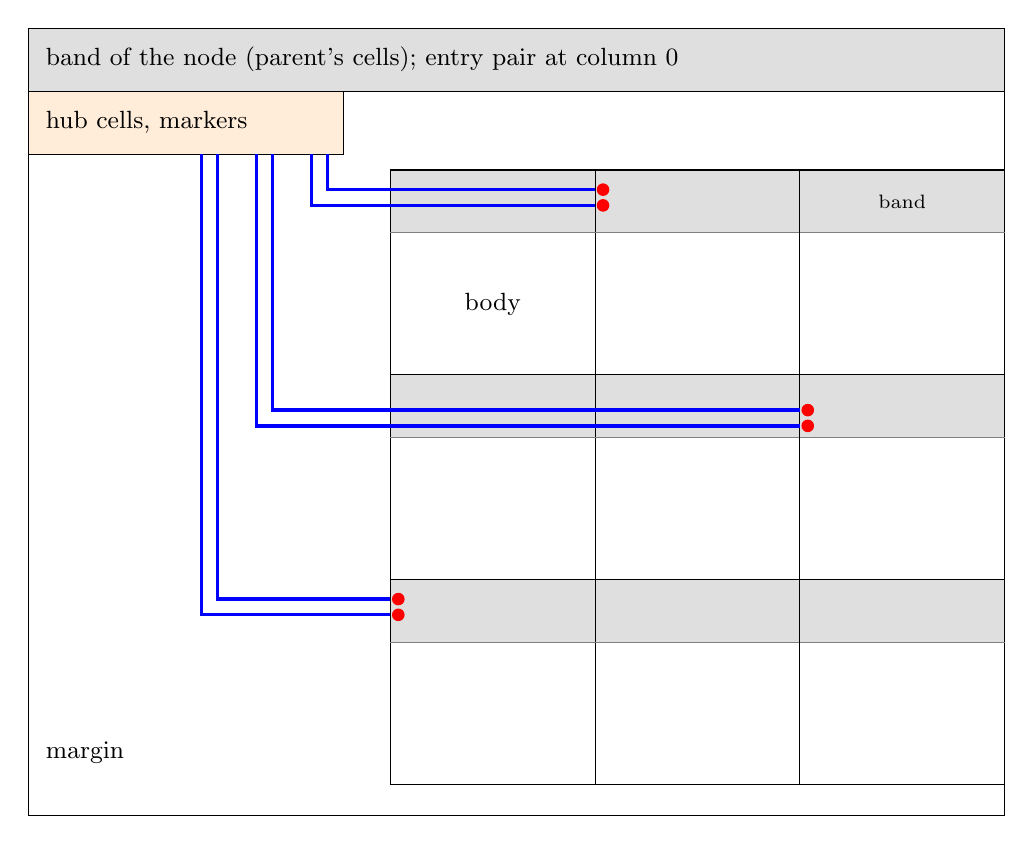
\begin{tikzpicture}[x=1mm,y=1mm,font=\small]
% node square and its band
\fill[gray!25] (0,92) rectangle (124,100);
\draw (0,0) rectangle (124,100);
\draw (0,92) -- (124,92);
\node[anchor=west] at (1,96) {band of the node (parent's cells); entry pair at column $0$};
% hub region
\fill[orange!15] (0,84) rectangle (40,92);
\draw (0,84) rectangle (40,92);
\node[anchor=west] at (1,88) {hub cells, markers};
% slots with their bands
\foreach \r/\top in {0/82,1/56,2/30}{
  \foreach \c in {0,1,2}{
    \pgfmathsetmacro{\x}{46+26*\c}
    \fill[gray!25] (\x,\top-8) rectangle (\x+26,\top);
    \draw (\x,\top-26) rectangle (\x+26,\top);
    \draw[gray] (\x,\top-8) -- (\x+26,\top-8);
  }
}
\node at (59,65) {body};
\node[font=\scriptsize] at (111,78) {band};
% lanes: spoke to slot (row 0, column 1)
\draw[blue,very thick] (36,84) -- (36,77.5) -- (72,77.5);
\draw[blue,very thick] (38,84) -- (38,79.5) -- (72,79.5);
\fill[red] (73,79.5) circle (0.8); \fill[red] (73,77.5) circle (0.8);
% lanes: spoke to slot (row 1, column 2)
\draw[blue,very thick] (29,84) -- (29,49.5) -- (98,49.5);
\draw[blue,very thick] (31,84) -- (31,51.5) -- (98,51.5);
\fill[red] (99,51.5) circle (0.8); \fill[red] (99,49.5) circle (0.8);
% lanes: spoke to slot (row 2, column 0)
\draw[blue,very thick] (22,84) -- (22,25.5) -- (46,25.5);
\draw[blue,very thick] (24,84) -- (24,27.5) -- (46,27.5);
\fill[red] (47,27.5) circle (0.8); \fill[red] (47,25.5) circle (0.8);
\node[anchor=west] at (1,8) {margin};
\end{tikzpicture}
\caption{A corner node, not to scale, with $3\times3$ instead of $b\times b$ slots and three of the $J$ spokes drawn.
Each slot holds a child: its top $W$ rows (shaded) are the child's band, the rest is the child's body. Each spoke's two
lanes (blue; the outer one is the export lane, the inner one the delivery lane) leave the hub, run down two margin columns of their own, then turn right along two rows of their own inside
the bands of their slot row, and end at the child's entry pair (red), in the first column of the child's square. Later spokes
use columns further left and rows further down (a child further right has its entry pair two rows lower in the band), so
no two lanes meet, and no lane enters a child's body. With $3\times3$ slots there would be $9$ spokes and $18$ lanes; the
figure shows $6$ of them.}\label{fig:corner}
\end{figure}

\begin{lemma}[corner layout]\label{lem:corner}
This is a star layout (Definition~\ref{def:layout}) whose body is the node's body. Moreover:
\begin{enumerate}[nosep]
\item $|X_j|+|Y_j|\le2\Delta_j+4b$, where $\Delta_j=\bar r_\xi+\bar c_{\kappa'}$ is the local distance from $o$ to the corner of slot
  $j$; also $|X_j|,|Y_j|\le2T$;
\item $h$, $|A_j|$ and the connector are $O(1)$, so $\cost_j=|X_j|+|Y_j|+O(1)$ and $c_{\rm wrap}=O(1)$;
\item $r=|\Res(P)|=O(T)$.
\end{enumerate}
\end{lemma}

\begin{proof}
\emph{Disjointness.} Spoke $j$ uses the margin columns $\gamma_j,\gamma_j+1$, which differ for different spokes. Its
horizontal part uses rows $y_j,y_j+1$ inside the band of slot row $\xi$, and $y_j$ is strictly increasing in
$j$ (consecutive slot rows are $T'>2b$ apart). The vertical part of a spoke $j'<j$ lies in columns to the right of $\gamma_j+1$ and ends at row
$y_{j'}+1<y_j$, so it does not meet the horizontal part of spoke $j$. Symmetrically, the vertical part of a spoke $j'>j$ lies in columns to the left of $\gamma_j$, and its
horizontal part, which crosses columns $\gamma_j,\gamma_j+1$, lies in rows $y_{j'}\ge y_j+2$, below the end (row $y_j+1$) of spoke $j$'s
vertical part. Horizontal parts run through the bands of slots, never through bodies, so loops avoid all
children. Loops avoid row $W+1$ (where $K,u,v,u'$ and the markers are) and row $W$ (where $w$, the access walks and
the connector run). The remaining conditions of Definition~\ref{def:layout}:
\begin{itemize}[nosep]
\item $A_j$ runs along row $W$ and then down column $\gamma_j<M_0$ through rows $W+1,W+2$. So it meets $L_j$ only at $x_j$ (the
  loop's vertical parts start at row $W+3$), and it avoids $K,u,v$ (row $W+1$, columns $>M_0$) and all children (rows $<W+4$).
\item The hub square contains $w$, $K,u,v,u'$ and every $H_j=(W+2,\gamma_j+1)$. The markers lie in row $W+1$, which no loop meets.
\item The connector uses column $0$ above row $W$ and row $W$ itself. It avoids the loops (columns $\ge1$, rows $\ge W+2$), the
  children (rows $\ge W+4$), $K,u,v$ (row $W+1$) and $e=(2\kappa,0)$, which lies above $z$.
\item $x_j,H_j,K,u,v,u',w$ and the markers lie in no child. The body (rows $\ge W$) excludes $e,z$.
\item The wrapper square is the square of side $h_w=W+M_0+6$ at the node's corner. It contains $e,z,w,K,u,v$, and it fits in
  the node's square since $T\ge W+M_0+12$; so do the hub square and the markers.
\end{itemize}
The definitions allow two harmless overlaps, which only matter for paths that restore everything: a child's connector
runs through the band of its slot, crossing the lanes of later spokes in the same slot row, and the hub square overlaps margin
loops and slot cells. Requests and double transpositions only promise net restoration, so neither matters.
\emph{Lengths.} $|X_j|=(y_j-W-1)+(\bar c_{\kappa'}-\gamma_j-1)+1$ and $|Y_j|=1+(\bar c_{\kappa'}-\gamma_j-1)+(y_j-W-3)$. Since
$y_j\le \bar r_\xi+2b$, this gives (1). (2) is immediate.
\emph{Reserve homes.} Own cells are the margin ($O(M_0T)$ cells), the four hub rows above the slots, the bands
of the slots ($b^2\cdot WT'\le bWT$ cells), and the leftover strips to the right of and below the slots, of
width less than $b+M_0$. The children's spare cells add $6J$. In total $O(T)$.
\end{proof}

\subsection{The cost recursion}

For a node $V$ with corner $o_V$ let $D_V=\sum_{x\in\cells(V)}d(o_V,x)$, and let $\operatorname{dp}(T)$ be the depth of
the tree below a node of side $T$: $0$ for a leaf, and $\operatorname{dp}(T')+1$ for a star.

\begin{theorem}\label{thm:tree}
There are constants $\Lambda_r,\Lambda_c$ such that every node $V$ of side $T\ge T_{\min}$, for a goal board whose blank is not in
the node's body, is a region with
\[
\rate_V\le \Lambda_rT,\qquad \base_V\le 2D_V+\Lambda_cT^2\bigl(\operatorname{dp}(T)+1\bigr).
\]
Moreover $\operatorname{dp}(T)\le\log_bT$.
\end{theorem}

\begin{proof}
Induction on $T$. For a leaf, $\rate=0$ and $\base=O(T^3)$; since $T<T_{\rm big}$, this is at most a constant times $T^2$, which $\Lambda_c$ absorbs.

Let $V=P$ be a star with children $Q_j$ of side $T'\le T/b$. By induction and Theorem~\ref{thm:star} it is a
region. We use Lemma~\ref{lem:corner} throughout.

\emph{Rate.} $\cost_{\max}\le4T+O(1)$, $\rate_{\max}\le \Lambda_rT'\le \Lambda_rT/b$ and $c_{\rm dx}=O(T)$, so
\[
\rate_P\le\bigl(4T+O(1)+\Lambda_rT/16\bigr)\cdot7+O(T)\le\tfrac{7}{16}\Lambda_rT+O(T)\le \Lambda_rT
\]
once $\Lambda_r$ is large enough. This uses $b>\mathcal H_J$: each level contracts the rate by the factor $\mathcal H_J/b<1$.

\emph{Base.} Let $\ell_j=|\cells(Q_j)|\ge\pop_j$. The terms of $\base_P$ in Theorem~\ref{thm:star} are bounded as follows.
\begin{itemize}[nosep]
\item $\sum_j\cost_j\pop_j\le\sum_j\ell_j(|X_j|+|Y_j|)+O(T^2)\le2\sum_j\ell_j\Delta_j+O(T^2)$, since $\sum_j\ell_j\le T^2$.
\item $\sum_j\cost_j(|X_j|+|Y_j|)\le J(4T+O(1))\,4T=O(T^2)$, and $J\cost_{\max}+\sum_j(2|A_j|+2|X_j|)=O(T)$.
\item $\rate_{\max}\sum_j(3+|X_j|+|Y_j|)\le (\Lambda_rT/b)\,J(4T+3)=O(\Lambda_rT^2)$.
\item $2(M+r)c_{\rm wrap}+2r\,c_{\rm dx}+O(T(r+6))=O(T^2)$, since $s_P=T$.
\item $\sum_j\base_j\le\sum_j2D_{Q_j}+J\Lambda_cT'^2(\operatorname{dp}(T')+1)\le2\sum_jD_{Q_j}+\Lambda_cT^2\operatorname{dp}(T)$, since $bT'\le T$.
\end{itemize}
Hence $\base_P\le2\sum_j(D_{Q_j}+\ell_j\Delta_j)+\Lambda_cT^2\operatorname{dp}(T)+\Lambda_0T^2$, where $\Lambda_0$ depends on $b$ and $\Lambda_r$ but not
on $\Lambda_c$.

\emph{Telescoping.} A cell $x$ of child $j$ has local coordinates $(\bar r_\xi+r',\bar c_{\kappa'}+c')$ with $r',c'\ge0$ its
coordinates in the child. So $d(o_P,x)=\Delta_j+d(o_{Q_j},x)$. The children's cells are disjoint cells of $P$, so
\[
D_P\ \ge\ \sum_j\sum_{x\in\cells(Q_j)}(\Delta_j+d(o_{Q_j},x))=\sum_j(\ell_j\Delta_j+D_{Q_j}).
\]
Therefore $\base_P\le2D_P+\Lambda_cT^2(\operatorname{dp}(T)+1)$, provided $\Lambda_c\ge \Lambda_0$ and $\Lambda_c$ also covers the leaves.

\emph{Depth.} $T'\le T/b$, and leaves have $T\ge T_{\min}\ge b$, so $\operatorname{dp}(T)\le\log_bT$.
\end{proof}

Informally: each tile whose home is in a node travels down the delivery lanes of all the ancestors of its
home, and each source leaves through their export lanes. At each level the lanes cost the distance to the next
corner, up to $O(1)$, and these distances add up along the chain of corners. The bound charges about $2D_V$ for
this, which is why the factor $2$ appears.

\section{The root and the main theorem}\label{sec:root}

\subsection{The central root}
Let $n$ be large and $T=\lfloor(n-5)/2\rfloor$, so the square $\mathcal S^*=[0,N^*)^2$ with $N^*=2T+5$ fits on
the board, with $N^*\in\{n-1,n\}$. Let $\chi=T+2$, so the cell $(\chi,\chi)$ is the centre of $\mathcal S^*$. For each
$j\in\{1,2,3,4\}$ with sign pair $(\iota_1,\iota_2)\in\{\pm1\}^2$, the \emph{reflection} $\rho_j$ maps
$(i,i')\mapsto(\chi+\iota_1(i-\chi),\,\chi+\iota_2(i'-\chi))$. It maps $\mathcal S^*$ onto itself, fixes the centre and preserves
adjacency and distances. We describe spoke $j$ in \emph{$j$-coordinates}: the cell with $j$-coordinates $(i,i')$ is the
board cell $\rho_j(i,i')$. Put $\mu=\chi+1$ and $\nu=\chi+3$. In $j$-coordinates:
\begin{itemize}[nosep]
\item child $j$ is a corner node of side $T$ with entry column $0$, in the placed square $(i,i')\mapsto\rho_j(\nu+i,\nu+i')$,
  $0\le i,i'<T$, which is the square $[\nu,N^*)^2$ in $j$-coordinates. So $e_j=(\nu,\nu)$ and $z_j=(\nu+1,\nu)$;
\item $x_j=(\mu,\mu)$ and $H_j=(\mu,\mu+1)$. The export queue is $(\mu+1,\mu),(\mu+2,\mu),(\mu+3,\mu),(\nu+1,\mu+1),z_j$, and the
  delivery queue is $e_j,(\nu,\mu+1),(\mu+1,\mu+1)$. The access walk is $(\chi,\chi),(\mu,\chi),x_j$.
\end{itemize}
In board coordinates, the hub square is the $7\times7$ square with corner $(\chi-2,\chi-2)$. The hub cells are $w=(\chi,\chi)$,
$K,u,v,u'=(\chi,\chi+1),\dots,(\chi,\chi+4)$ and the four $H_j$. The entry pair is $e^*=(\chi,\chi-2)$, $z^*=(\chi,\chi-1)$, the
connector is $z^*\to w$, and the markers are $(\chi,\chi+5+i)$, $0\le i<6$. The body is the whole board except $e^*,z^*$.
The wrapper square is the hub square, and the square of the root is the whole board.

\begin{lemma}\label{lem:rootlayout}
This is a star layout with $J=4$ in which every loop, access walk and connector has length $O(1)$, and
$r=O(n)$.
\end{lemma}

\begin{proof}
Call row $\chi$ and column $\chi$ of $\mathcal S^*$ the \emph{middle row} and \emph{middle column}. A cell whose two $j$-coordinates are at least $\mu=\chi+1$ lies, on the board, strictly on one side of the middle
row and of the middle column, in the quarter determined by $(\iota_1,\iota_2)$. The loop, $x_j$, $H_j$ and the child of spoke $j$
consist of such cells, so different spokes are disjoint, and none of them meets the middle row or the middle column. The
middle row holds $w,K,u,v,u'$, the entry pair and the markers. The access walk passes through $\rho_j(\mu,\chi)$, which is on the
middle column but on no loop. The hub square, which is also the wrapper square, contains $w,K,u,v,u'$, the entry pair and every $H_j=\rho_j(\mu,\mu+1)$, which has
board coordinates $(\chi\pm1,\chi\pm2)$. The access walk meets its loop only at $x_j$ and avoids $K,u,v$. The connector consists of
$z^*$ and $w$ alone. The markers lie on the middle row. The own cells are the central cross of
width $5$, the four children's bands ($O(T)$ cells each), and possibly the last row and column. So $r=O(n)$.
\end{proof}

Let $\tau$ be the target board, with blank at the corner $\theta=(n-1,n-1)$, and let the goal
$G'$ be $\tau$ with the contents of $z^*$ and $\theta$ exchanged. So $G'$ has its blank at $z^*$, which is in
no cell of $P^*$ or of any node below it. Hence $G'(x)\ne0$ for every home $x$ of every node, as frames require. The root $P^*$ is this star layout with goal $G'$.

\begin{lemma}\label{lem:rootbudget}
$P^*$ is a region with $\base_{P^*}+\rate_{P^*}\le 8T^2(T-1)+4\Lambda_cT^2(\log_bT+1)+O(n^2)$.
\end{lemma}

\begin{proof}
Apply Theorem~\ref{thm:star} with $J=4$, $\mathcal H_4<3$. Everything except the children's bases is $O(n^2)$:
$\cost_j=O(1)$, $\pop_j\le T^2$, $|X_j|,|Y_j|=O(1)$, $\rate_{\max}\le \Lambda_rT$ (Theorem~\ref{thm:tree}),
$c_{\rm dx}=O(n)$, $r=O(n)$, and $\rate_{P^*}=O(n)$. By Theorem~\ref{thm:tree}, $\base_j\le2D_{Q_j}+\Lambda_cT^2(\log_bT+1)$,
and $D_{Q_j}\le\sum_{0\le r',c'<T}(r'+c')=T^2(T-1)$.
\end{proof}

\subsection{Driving the root}

\begin{lemma}[driver]\label{lem:driver}
Let $R$ be a region with entry pair $(e_R,z_R)$, on a board with the blank at $z_R$, no blank in $\cells(R)$, and every core and reserve home of
$R$ holding a goal tile of $R$. Then a path of length at most $\base_R+\rate_R$ makes every home of $R$ hold its goal,
returns the blank to $z_R$, and changes no cell outside $\cells(R)\cup\{e_R\}$.
\end{lemma}

\begin{proof}
Start $R$ (allowance $0$), and raise its allowance to $1$ by~\ref{R:relax}. Its sources are the tiles in its homes, all goal tiles. Make a helper request with the tile at
$e_R$ (which is not the blank). The output is a source, hence a goal tile of $R$, and it is now outside $R$. Feed it straight
back as a core or reserve arrival according to whether its home is a core or a reserve home. Each such arrival again outputs a source, while any remain,
and we feed it back too. The lead is $1$ after the first request and stays $1$ while sources remain, so allowance $1$
suffices. After the helper request and $M+r$ goal arrivals, every source has been handed out and received back,
so $a_c=M$ and $a_r=r$, and $R$ finishes. The total work is at most $\base_R+\rate_R\cdot1$.
\end{proof}

\subsection{Proof of Theorem~\ref{thm:main}}

\begin{proof}
\emph{Solving to the target.} Let $B$ be connected to $\tau$.
\begin{enumerate}[nosep]
\item Move the blank to $z^*$ (Lemma~\ref{lem:elbow}): at most $2n$ moves.
\item Let $\mathcal K$ consist of $0$ and the seven tiles $G'(x)$ for $x$ a marker or $e^*$, and let
  $\mathcal R=\text{markers}\cup\{e^*,z^*\}$. Gather $\mathcal K$ into $\mathcal R$ (Lemma~\ref{lem:gather}): $O(n)$ moves. Now every
  home of $P^*$ (every cell other than the markers, $e^*$ and $z^*$) holds a tile not in $\mathcal K$, that is, a goal tile
  of $P^*$.
\item Drive $P^*$ (Lemma~\ref{lem:driver}): at most $8T^2(T-1)+4\Lambda_cT^2(\log_bT+1)+O(n^2)$ moves. Afterwards the
  board agrees with $G'$, hence with $\tau$, outside $\mathcal R\cup\{\theta\}$, and the blank is at $z^*$.
\item Move the blank to $\theta$ (Lemma~\ref{lem:elbow}): at most $2n$ moves, changing at most $2n$ cells.
\item The board now differs from $\tau$ on at most $2n+9$ cells, has its blank at $\theta$, and is connected to $\tau$.
  Lemma~\ref{lem:cleanup} finishes in $O(n^2)$ moves.
\end{enumerate}
Since $2T\le n$, $8T^2(T-1)\le n^3$. The total is at most $n^3+O(n^2\log n)$.

\emph{Arbitrary pairs.} Let $B$ and $B'$ be connected. Move the blank of $B'$ to $\theta$ by a path $\zeta$ of at most
$2n$ moves, giving $B''$. Let $\sigma$ be the renaming of tiles that turns $B''$ into $\tau$; it fixes $0$.
Moves do not depend on tile names, so the renamed board $\sigma(B)$ is connected to $\sigma(B'')=\tau$. The path
from $\sigma(B)$ to $\tau$ found above, applied to $B$, leads to $B''$, and $\zeta$ reversed leads on to $B'$. The cost is at
most $n^3+O(n^2\log n)+2n$.
\end{proof}

\begin{thebibliography}{9}
\bibitem{johnsonstory} W.~W.~Johnson and W.~E.~Story, Notes on the ``15'' puzzle,
\emph{American Journal of Mathematics} \textbf{2} (1879), 397--404.
\bibitem{parberry} I.~Parberry, A real-time algorithm for the $(n^2-1)$-puzzle,
\emph{Information Processing Letters} \textbf{56} (1995), 23--28.
\end{thebibliography}

\end{document}
